\documentclass[final]{beamer}
\usetheme{Boadilla}
\usepackage{siunitx}
\usepackage{amsmath}
\usepackage{graphicx}
\usepackage[labelformat=empty]{caption}
\usepackage{verbatim}
\usepackage[orientation=portrait,size=a2]{beamerposter}
\usepackage[absolute,overlay]{textpos}

\title{Optimising the design of buffer preparation in bioprocessing facilities}
\institute[UCD]{University College Dublin}
\date{\today}
\subtitle{MSc in Business Analytics (Part Time) 2015--2017}
\author{Sean Tully}



%==the poster content
\begin{document}
    \begin{frame}[t]
        \begin{columns}
            \column{0.15\textwidth}
                \begin{figure}
                    \centering
                    
\includegraphics[angle=0,scale=0.08]{ucd_logo.png}
                \end{figure}
            \column{0.7\textwidth}
            %\centering MSc in Business Analytics -- Dissertation\\
            \centering
            \vspace{0.5cm}
            
            \Huge{\textbf{Optimising the design of buffer preparation in
                 bioprocessing facilities}}
                 
            \huge \emph{Author: Sean Tully \quad Supervisor: Prof. Michael
                O'Neill}
            \column{0.15\textwidth}
                \begin{figure}
                    \centering
                    
\includegraphics[angle=0,scale=0.08]{ucd_logo.png}
                \end{figure}
        \end{columns}
        
        \vspace{0.5cm}
        
        \huge
        \begin{columns}[t]
            \column{0.47\textwidth}
                \begin{block}{\huge Aim}
                    To develop a methodology and software tool for finding the
                    optimum number, size and assignment of buffer preparation
                    vessels in the design of a large-scale bioprocess facility.
                \end{block}
                \begin{figure}
                    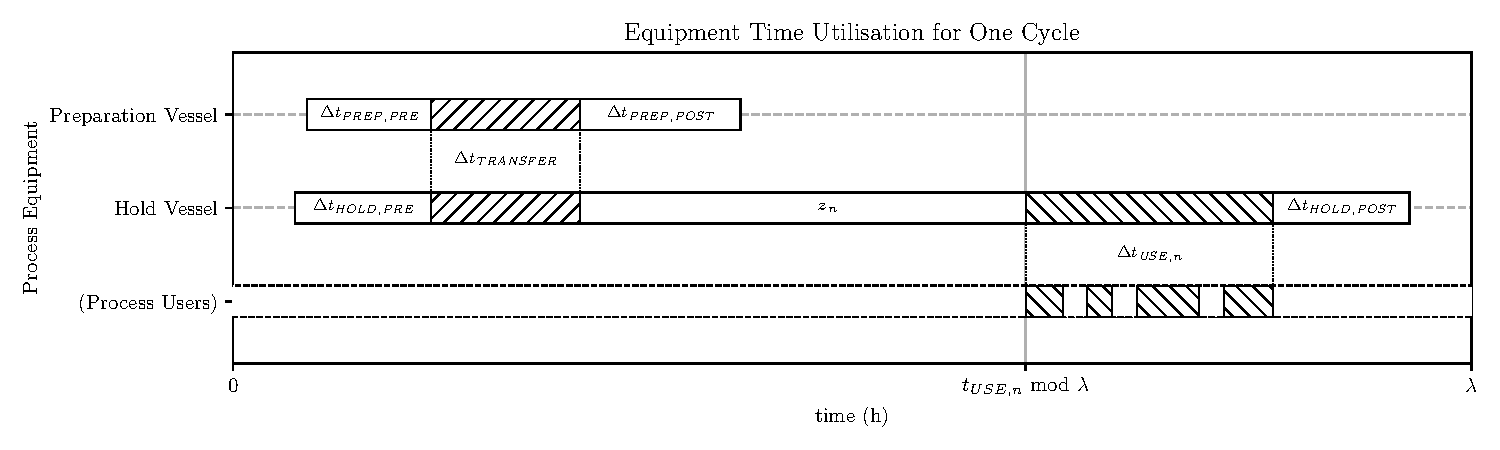
\includegraphics[width=\textwidth]{./../figures/explanatory.pdf}
                \end{figure}
                \begin{block}{\huge Methodology}
                    The problem was described as a mixed-integer linear
                    programming problem and solved using several linear
                    programming packages via the PuLP python library.
                 \end{block}
                \begin{block}{\huge Basic Problem -- no scheduling}
                    \begin{itemize}                 
                        \item The objective function (to be minimised) is the
                            total cost of preparation vessels.\\
                        \item Each buffer must be prepared in a particular 
                            \emph{slot} (a notional space that may contain a
                            vessel).
                        \item Each slot may contain at most one vessel.
                        \item Each vessel must be adequately sized.
                        \item{Preparation vessels must not be over-utilised}
                    \end{itemize}
                \end{block}
                \begin{block}{\huge Complete Problem -- with scheduling
                    constraints}
                    The following constraints are added to the basic problem:
                    \begin{itemize}                 
                        \item Buffer hold procedure must be shorter than cycle
                            time.
                        \item Preparation procedures mustn't clash
                    \end{itemize}
                \end{block}
                \begin{block}{\huge Secondary Problem -- goal programming}
                    Find an improved result with minimised buffer hold times.
                    \begin{itemize}
                        \item Constrain total vessel cost to be equal to the
                            objective function value from the complete problem.
                        \item Set the minimisation of buffer hold durations as
                            the new objective.
                    \end{itemize}
                \end{block}
                \begin{block}{\huge Implementation}
                    \begin{itemize}
                        \item Programming carried out in python.
                        \item LP problems solved via the PuLP API.
                        \item The CPLEX, Cbc and GLPK solvers were used.
                        \item The matplotlib library was used for generating
                            plots.
                    \end{itemize}
                \end{block}
            \column{0.47\textwidth}
                \begin{block}{\huge Results -- Complete Model}
                    Block text
                \end{block}
                TODO: lots of grpahics
                Less text
                Business Case
                Academic Contribution
                Conclusions
                Scope for further work
                \begin{figure}
                    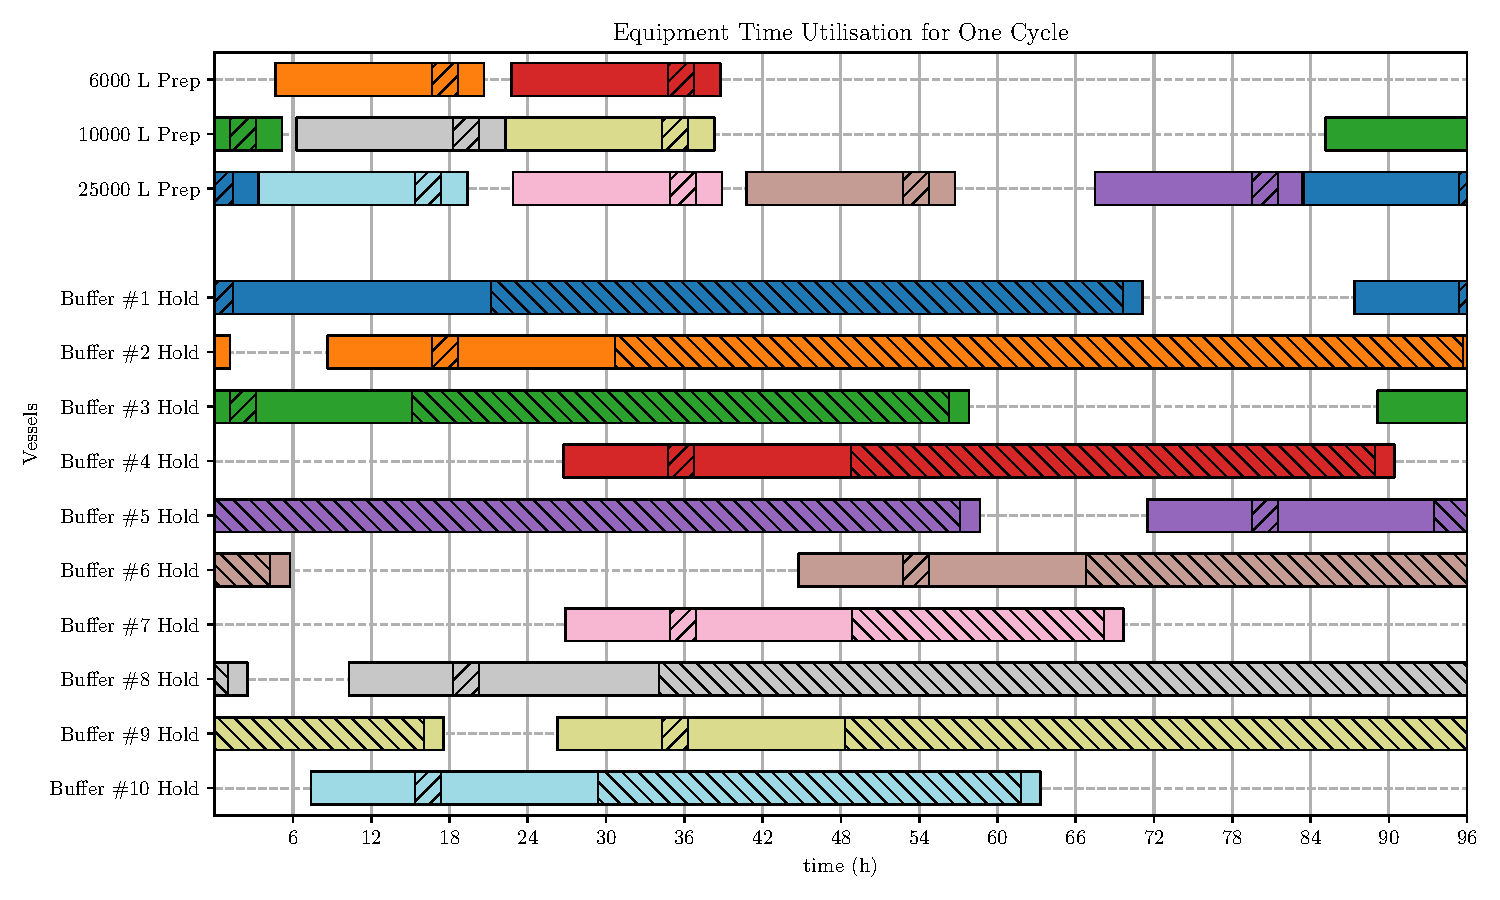
\includegraphics[width=0.99\textwidth]{./../figures/plot2.pdf}
                    \captionsetup{justification=centering}
                    \caption{\Large Steady-State Equipment Time Utilisation
                    plot showing a feasible schedule for a random problem with
                    12 buffers, for a single cycle, with minimal buffer vessel
                    cost and hold times minimised.}
                \end{figure}
                \begin{figure}
                    \includegraphics[width=0.7\textwidth]{timings.pdf}
                    \caption{\Large Solution duration as a function of problem
                        size and solver selection.}
                \end{figure}
        \end{columns}
    \end{frame}
\end{document}
